
%(BEGIN_QUESTION)
% Copyright 2011, Tony R. Kuphaldt, released under the Creative Commons Attribution License (v 1.0)
% This means you may do almost anything with this work of mine, so long as you give me proper credit

This solvent storage tank is kept heated to 95 degrees F by a steam heat exchanger inside the tank.  Steam is admitted to the exchanger ``loop'' through temperature control valve TCV-105, and exits the loop through a steam trap:

$$\includegraphics[width=15.5cm]{i0006rx01.eps}$$

The tank's temperature control system is interesting, in that there is neither a temperature transmitter nor a temperature controller, just a self-actuated temperature control valve.  The line connecting TCV-105's actuator with the tank (the one with the ``X'' symbols along its length) is a {\it capillary tube} filled with a liquid that expands with temperature.  The far end of this tube (inside the tank) terminates in a sealed metal bulb, so there is no way the fluid inside the tube can escape.

\vskip 10pt

First, explain how this temperature control system functions during normal operation.

\vskip 10pt

Next, identify what you would have to mechanically adjust on TCV-105 in order to raise the temperature setpoint for the storage tank.

\vskip 10pt

Finally, identify the fail-safe state of this temperature control valve.

\vskip 20pt \vbox{\hrule \hbox{\strut \vrule{} {\bf Suggestions for Socratic discussion} \vrule} \hrule}

\begin{itemize}
\item{} Identify the meaning of the dashed line inside the solvent storage tank.  Does this mean the same thing as the dashed lines outside of the tank?  How can we tell one way or the other?
\end{itemize}

\underbar{file i03444}
%(END_QUESTION)





%(BEGIN_ANSWER)

{\bf Partial answer:}

\vskip 10pt

TCV-105 {\it fails open} (assuming the failure is a leak in the capillary tube system.
 
%(END_ANSWER)





%(BEGIN_NOTES)

Pressure generated inside the sensing bulb due to temperature acting on the enclosed fluid presses against the valve's diaphragm to shut it off, thereby decreasing steam flow as vessel temperature increases.

\vskip 10pt

The control valve's spring load adjustment would serve as the temperature setpoint, since this will ``bias'' the control valve to require different amounts of filled-system fluid pressure for any given \% opening.

\vskip 10pt

Given that increased bulb pressure shuts off this valve, a failure of this filled-bulb pressure will cause the steam valve to open wide, possibly overheating the vessel.





\vskip 20pt \vbox{\hrule \hbox{\strut \vrule{} {\bf Virtual Troubleshooting} \vrule} \hrule}

This question is a good candidate for a ``Virtual Troubleshooting'' exercise.  Presenting the diagram to students, you first imagine in your own mind a particular fault in the system.  Then, you present one or more symptoms of that fault (something noticeable by an operator or other user of the system).  Students then propose various diagnostic tests to perform on this system to identify the nature and location of the fault, as though they were technicians trying to troubleshoot the problem.  Your job is to tell them what the result(s) would be for each of the proposed diagnostic tests, documenting those results where all the students can see.

During and after the exercise, it is good to ask students follow-up questions such as:

\begin{itemize}
\item{} What does the result of the last diagnostic test tell you about the fault?
\item{} Suppose the results of the last diagnostic test were different.  What then would that result tell you about the fault?
\item{} Is the last diagnostic test the best one we could do?
\item{} What would be the ideal order of tests, to diagnose the problem in as few steps as possible?
\end{itemize}











\vfil \eject

\noindent
{\bf Summary Quiz:}

What will happen to the temperature inside the solvent storage tank if the capillary tube ruptures?

$$\includegraphics[width=15.5cm]{i03444x01.eps}$$






%INDEX% Process: solvent storage tank (realistic P&ID shown)

%(END_NOTES)


